\section{First start of the \emph{Reprotool}}
When you run \emph{Reprotool} for the first time, an \emph{eclipse} welcome page will be displayed. Close this page.
The next thing you need to set up is to select the \emph{Reprotool} perspective in the \emph{eclipse IDE}.
Now open the \emph{Open Perspective dialog} with the
\begin{verbatim}
 Window / Open Perspective / Other
\end{verbatim}
menu command. Now select \emph{Reprotool} and click OK. The \emph{Reprotool} perspective will now be showed in your \emph{eclipse}
workbench. It looks like this:

\begin{figure}[ht]
  \centering
  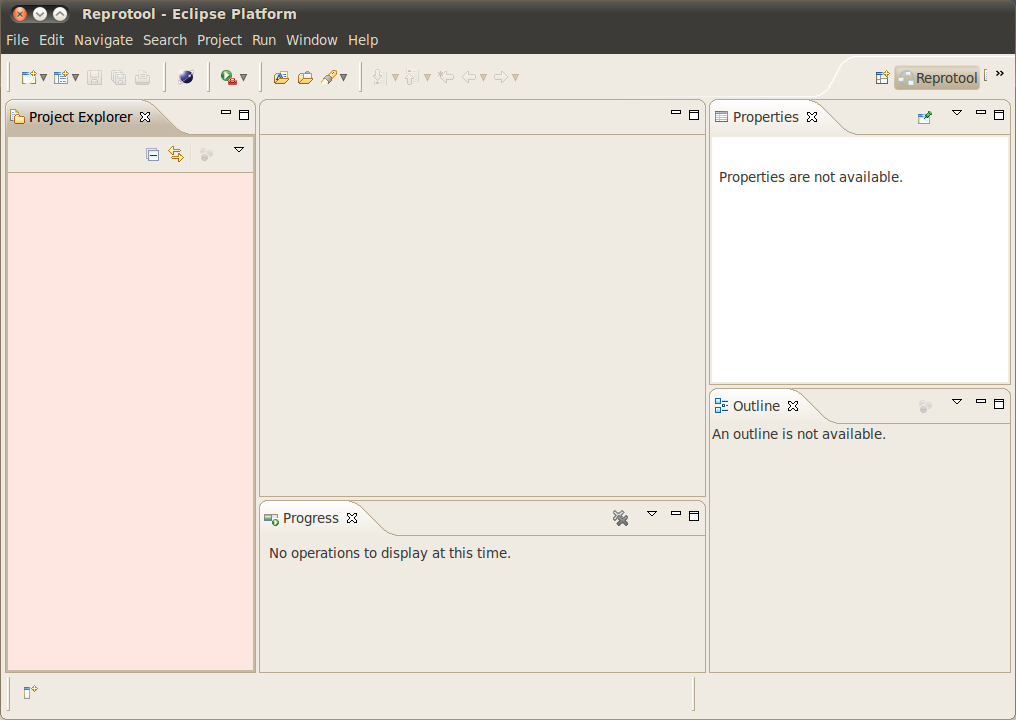
\includegraphics[height=280pt]{images/reprotoolPerspective}
  \caption{Empty \emph{Reprotool} perspective}
  \label{fig:reprotoolPerspective}
\end{figure}

